\chapter{Marco teórico}\label{marcoteorico}
\section{Antecedentes}\\ \label{sec:antecendentes}

El reconocimiento automático de placas vehiculares es muy importante en los sistemas de control de tránsito. Estos sistemas implementan algoritmos que permiten analizar imágenes digitales utilizando técnicas de reconocimiento óptico de caracteres (del inglés, \textit{Optical character recognition} - OCR) \cite{noaman2012optical}. Para lograr esto, se usa con frecuencia la implementación de inteligencia artificial, que puede incluir componentes como redes neuronales, algoritmos genéticos, lógica difusa u ordenamiento estadístico \cite{Calderon2017}. En muchos países se realiza el reconocimiento automático de placas vehiculares para el acceso al estacionamiento, rastreo de vehículos, control de fronteras, conteo de vehículos e identificación policial con fines de seguridad. Esto ha sido fruto de algunas de las siguientes investigaciones: 

\begin{itemize}
    \item Patel et \textit{al} \cite{patel2013automatic} proponen un sistema con técnicas de aprendizaje supervisado en redes neuronales artificiales convolucionales, utilizando la plataforma Caffe y sus librerías, así como también librerías en OpenCV y scripts desarrollados en Python.
    \item Shivakumara et \textit{al} \cite{shivakumara2018cnn} combinaron CNN y RNN para reconocer imágenes de matrículas mediante clasificación. Para la clasificación de imágenes de matrículas privadas y públicas, el método propuesto exploró la separación de primer plano y fondo, y luego la agrupación de una nueva manera. Los resultados experimentales en la clasificación mostraron que la clasificación propuesta es mejor que los métodos existentes en términos de tasa de clasificación.
    \item En México se tienen estudios similares desde el año 2010 con el proyecto de Montiel et \textit{al} \cite{montiel2010reconocimiento}. Este autor propuso un sistema de reconocimiento de placas de los vehículos en la ciudad de México usando RNC. Los resultados experimentales obtenidos en condiciones reales de operación muestran que el sistema propuesto presenta un acierto del 99.84\% con caracteres que se usaron en el proceso de entrenamiento y un 98.78\% con caracteres que no fueron utilizados en el proceso de entrenamiento.
    \item Cika et \textit{al} \cite{cika2011detection} y Patel et \textit{al} \cite{patel2013automatic} usan algoritmos de segmentación múltiple para la identificación de la placa del vehículo, esto implica el uso doble de carga computacional, debido a que la comparación de patrones se usa en orden para dividir el área de la placa y paralela a esta, luego se implementan redes neuronales para identificar a cada personaje.
    \item Chu et \textit{al} \cite{chu2019sistema} implementaron un sistema de reconocimiento de placas vehiculares en un hospedaje ``Suites Recreo - 2019”\ en Perú. Se usó la metodología de desarrollo XP utilizando el algoritmo Clasificador Haar Cascade, motor de reconocimiento de caracteres Tesseract, librerías de visión artificial Opencv, EmguCV y Aforge.NET, el sistema gestor de base datos Mysql y el entorno de desarrollo Visual Studio 2015. Se obtuvo que el tiempo promedio de registro de vehículos sin el sistema fue de 47.27 segundos y con el sistema implementado fue de 15.10 segundos.
    \item Espinoza et \textit{al} \cite{espinoza2015desarrollo} desarrollaron un sistema de reconocimiento de placas vehiculares mediante el análisis de imágenes digitales. El uso de la interfaz gráfica web presentó una tasa de reconocimiento del 91\%.
    \item Alvarez et \textit{al} \cite{alvarez2014analisis} diseñaron un sistema de reconocimiento de placas vehiculares que permitió identificar los vehículos que ingresan al parqueadero de la Universidad Politécnica Salesiana. Este proceso usó una cámara conectada al sistema de visión artificial. Presentó un 94\% de acierto en el reconocimiento de placas.
    \item En Perú, Rojas et \textit{al} \cite{rojas2017desarrollo}, desarrollaron sistema de reconocimiento de placas en \textit{JAVAanpr} y estudiaron su influencia en la detección de vehículos robados en la municipalidad San Isidro. Los autores indican que al realizar la búsqueda de vehículos robados con la policía por los medios tradicionales no se llega ni al 20\% de efectividad además de tener un alto costo operativo, sin embargo aplicando inteligencia artificial, la efectividad de este sistema es del 96\%. 
    \item Diferentes empresas e instituciones Ecuatorianas tienen un prototipo para el acceso vehicular, de esta manera reemplazan el operador humano que se encargaba de la vigilancia, esto mediante técnicas de visión artificial valiéndose de insumo los vídeos de vigilancia de acceso. Así como tienen software y hardware comerciales de reconocimiento de placas, como: Transcore, Intellisoft Parking, FxCAM, IBW2000, 3LPR.
\end{itemize}

Por otro lado, en Colombia contamos con muy pocas investigaciones en este tema, la mayoría son tesis de pregrado y postgrado, y no fueron implementados considerando los recursos físicos como la memoria RAM, la memoria no volátil o la capacidad de procesamiento limitado. A continuación se mencionan algunos de estos estudios: 

\begin{itemize}
    \item Estudiantes del programa de ingeniería electrónica de la Pontificia Universidad Javeriana, desarrollaron un software de demostración para el reconocimiento de caracteres impresos en Turbo C++ \cite{TrabajodeGrado2}y en 2005, fue desarrollado otro sistema en la plataforma Microsoft.net con base en las funciones y clases del conjunto de librerías Open source Computer Visión\cite{TrabajodeGrado}. Por su parte y como una iniciativa propia, la Universidad de los Andes desarrolló un sistema que utiliza sistemas de visión artificial para el tratamiento de imágenes con el fin de automatizar este proceso en sus instalaciones \cite{Uniandes}.
    \item González \& Col. (2008) crearon el software RAMVP V1.0 que trabaja con la plataforma MatLab. La investigación de estos autores combinaron distintos métodos de procesamiento de imágenes. El primero, extraía información de una escena paso a paso; y el segundo fue  una implementación preliminar de redes neuronales artificiales en el reconocimiento de patrones. Cientes de que puede abrir nuevos campos, el software creado trabaja con otro tipo de metodología\cite{trabajodegrado3}.
    \item Recientemente, Vasquez \& Melo (2018) diseñaron un sistema de conteo y reconocimiento automático de placas vehiculares, para el parqueadero de la sede principal de la Universidad Cooperativa de Colombia seccional Bogotá. También fue utilizado el software matemático MATLAB\cite{melo2019sistema}
    \item La investigación desarrollada por Calderón et \textit{al}\cite{Calderon2017} es el primero  en Colombia que propone abiertamente un reconocimiento del número de matrícula utilizando solo componentes de software. El sistema propuesto es integrado con recursos limitados y con capacidad de procesamiento mixto, específicamente usando el ZedBoard, que incluye un dispositivo Zynq 7000 Xilinx device. Es importante mencionar que Calderón et \textit{al}  \cite{Calderon2017} utiliza un método similar al propuesto en este trabajo. Sin embargo, los autores implementan una red neuronal poco compleja (capa de entrada: 128, capa oculta: 15 y capa de salida: 6 neuronas) programado en un sistema informático Linux, con costos computacionales relativamente altos (software y hardware), y una cámara estándar de detección.
\end{itemize}

\section{Marco conceptual}

Las competencias necesarias para llevar a cabo el presente trabajo, se relacionan con el campo del Deep Learning, específicamente todo lo relacionado con la comprensión de las Redes Neuronales Convolucionales. Desde como construir una arquitectura desde cero hasta la implementación de la transferencia de aprendizaje. Además, entender las diferentes métricas para evaluar su rendimiento. También, fue necesario adquirir competencias en las diferentes herramientas computacionales para su implementación. 
Por otro lado, para la construcción de la base de datos fue necesario entender algunas técnicas de segmentación y etiquetado propias del procesamiento de imágenes y conocer las herramientas computacionales para realizar tal tarea. 
El marco conceptual que se describe a continuación está relacionado con todos los conceptos básicos que permitieron adquirir todas las competencias antes mencionadas.

\subsection{Machine Learning}

Una regla de aprendizaje no es más que un procedimiento por el cual se modifican los pesos y el “bias” de la red. El propósito principal de que una red aprenda es que sea capaz de resolver una tarea que antes no podía (sabía) resolver. Existen muchos tipos de métodos de aprendizaje, pero los principales son: aprendizaje supervisado, aprendizaje no supervisado y aprendizaje reforzado\cite{Algoritmos}.

\begin{itemize}
    \item \textbf{Aprendizaje supervisado}: El aprendizaje se realiza mediante un entrenamiento controlado por un agente externo (supervisor, maestro) que determina la respuesta que debería generar la red a partir de una entrada determinada. El supervisor controla la salida de la red y en caso de que esta no coincida con la deseada, se procederá a modificar los pesos de las conexiones, con el fin de conseguir que la salida obtenida se aproxime a la deseada. Para lograr lo anterior, la red es provista con una seria de ejemplos que indican como la red debe funcionar.
    \item \textbf{Aprendizaje reforzado}: La diferencia con el caso anterior, es que cada entrada está asociada a una puntuación. Esta puntuación es una medida del rendimiento de la red ante varias secuencias de entrada. Dependiendo de la nota, la red actuará de una manera u otra: sí la nota es baja, el algoritmo de aprendizaje modificará en gran medida los elementos de la matriz de pesos y el bias, si la nota es media, los modificará más suavemente, y si es buena, los mantendrá o apenas modificará.
    \item \textbf{Aprendizaje no supervisado}: Son aquellos en los que no disponemos de una batería de ejemplos previamente clasificados, si no que la matriz de peso y el bias son modificadas en respuesta solo a las entradas de la red, ya que no existen objetivos. De esta manera, los algoritmos trabajan agrupando, es decir, la red aprende a categorizar los patrones de entrada en una serie finita de clases, según las propiedades de los ejemplos buscando la similitud.
\end{itemize}

\subsubsection{Algoritmo de aprendizaje supervisado \textit{backpropagation}}

El algoritmo de aprendizaje de estas redes permite extraer los atributos o características de cada clase a partir de un conjunto de datos de entrenamiento previamente clasificado. Estos atributos son los pesos de las diferentes neuronas de la red, y sus valores se calculan de manera iterativa mediante un método de aprendizaje supervisado denominado backpropagation o “propagación de errores hacia atrás”\cite{lecun1989backpropagation,chauvin1995backpropagation}. El algoritmo consta de dos etapas que se repiten interactivamente por cada elemento del conjunto de entrenamiento \cite{hecht1992theory}:
\begin{itemize}
    \item Etapa 1: Se calcula la clase a la que pertenece el ejemplar de entrada según los valores actuales de los pesos de la red. Una vez clasificado, el algoritmo determina la validez de dicha clasificación mediante una función de error.
    \item Etapa 2: El algoritmo propaga el error hacia atrás a todas las neuronas de la red que han contribuido a la clasificación del ejemplar, recibiendo cada una la “porción” del error correspondiente en función de su aportación, para que actualicen los pesos proporcionalmente, de tal manera que los nuevos valores reduzcan el error de clasificación. 
\end{itemize}
El algoritmo empleado para esta optimización suele ser el de descenso del gradiente. La combinación de ambos métodos; propagación hacia atrás y descenso del gradiente tiene como objetivo minimizar la función de error \cite{marin2013introduccion}.

\subsection{Redes Neuronales Artificiales - RNA}

Las redes neuronales biológicas son inmensas redes de neuronas interconectadas mediante procesos químicos y eléctricos. Todas esas neuronas conectadas entre sí le permiten al ser humano ser capaz de sentir, memorizar, aprender, etc. las redes neuronales artificiales (RNA) o perceptrón surgen del intento de imitar el comportamiento de las neuronas cerebrales usando software y hardware ultra avanzados \cite{marin2013introduccion}. Las características principales de las RNA son las siguientes:

\begin{itemize}
    \item Auto-Organización y Adaptabilidad: Utilizan algoritmos de aprendizaje adaptativo y auto-organización, por lo que ofrecen mejores posibilidades de procesado robusto y adaptativo.
    \item Procesado no Lineal: Aumenta la capacidad de la red para aproximar funciones, clasificar patrones y aumenta su inmunidad frente al ruido. 
    \item Procesado Paralelo: Normalmente se usa un gran número de nodos de procesado, con alto nivel de interconectividad.
\end{itemize}

Las RNA consisten de un gran número de elementos simples de procesamiento llamados nodos o neuronas que están organizados en capas. Cada neurona está conectada mediante enlaces de comunicación, cada uno de los cuales tiene asociado un peso. Estos pesos representan la información que será usada por la red neuronal para resolver un problema determinado, Matich et \textit{al} \cite{matich2001redes}.\\ 

\begin{figure}[H]
    \centering
    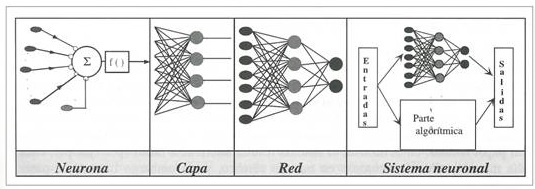
\includegraphics[width=1\linewidth]{imagenes/perceptron.jpg}
    \caption{Estructura jerárquica de una red neuronal artificial (RNA)}
    \label{fig:Estructura jerárquica de una red neuronal artificial (RNA)}
\end{figure}

\textbf{La figura \ref{fig:Estructura jerárquica de una red neuronal artificial (RNA)}} nos muestra en detalle cada elemento que forma a una RNA, una neurona, la capa, la red y todo el sistema conformado por cada uno de estos elementos. Hay tres fases en la modelización con redes neuronales \cite{marin2013introduccion}:

\begin{itemize}
    \item \textbf{Fase de entrenamiento}: Se usa un conjunto de datos para determinar los pesos que definirán el modelo de la red neuronal.
     \item \textbf{Validación}: Para evitar el problema del sobreajuste, se usa un conjunto de datos diferentes a los de entrenamiento, el grupo de validación, que permita controlar el proceso de aprendizaje.
    \item \textbf{Fase de Prueba}: En la fase anterior, el modelo puede que se ajuste demasiado a las particularidades presentes en los patrones de entrenamiento, perdiendo su habilidad de generalizar su aprendizaje a casos nuevos (sobreajuste).
\end{itemize}    
Usualmente con una única neurona no será suficiente para resolver la mayoría de problemas prácticos. Para resolver problemas más complejos se tendrá que hacer un uso conjunto de muchas de estas neuronas simples, dando lugar a una verdadera red neuronal, en la que se tendrán cientos o incluso miles de neuronas. Es ahí donde aparece el concepto de capa, que es la agrupación de todas estas neuronas en varios conjuntos dentro de la red neuronal completa \cite{duran2017redes}. 
    
\begin{figure}[H]
\centering
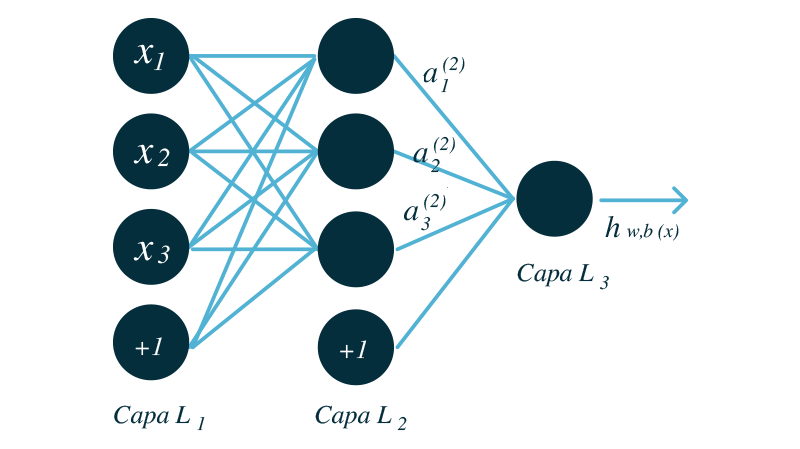
\includegraphics[width=0.7\linewidth]{imagenes/3_capas.png}
\caption{Estructura de una red neuronal de 3 capas}
\label{fig:3_CAPAS}
\end{figure}

La figura \ref{fig:3_CAPAS} es una muestra de una red neuronal artificial con una sola capa oculta, una de entrada y una capa de salida, para conformar así, 3 capas en sus sistema neuronal.\\
Si tenemos $n_{l}$ capas en una red neuronal, la l-ésima capa se denominará $L_{l}$, en ese sentido, la capa de entrada de la red será $L_{1}$, así mismo la capa de salida de la red será $L_{n}__{l}$. También se tendrá que $W_{ij}^{l}$ será el peso asociado a la conexión entre el elemento j de la capa l y el elemento i de la capa l+1, además, es la bias $b_{i}^{l}$ asociada con el elemento i de la capa l+1. Por último, se usará $a_{i}^{l}$ para denotar la activación (es decir, el valor de salida) del elemento i en la capa l. \\
El vector de entrada \textbf{X} está conectado con cada una de las
neuronas a través de la matriz de pesos \textbf{W}, es decir cada neurona de cada capa está conectada con todos los elementos de la capa que le precede. Este tipo de capas se denomina totalmente conectada o, en inglés, full connected. Además, cada neurona posee su propia bias. Todo esto supone que la salida de la neurona $n_{i}$ vendrá dada por la suma ponderada entre cada elemento de la entrada multiplicado por su correspondiente elemento de la matriz de pesos y la bias, en otras palabras, es:
\begin{center}
    $a_{1}^{2}= f({W_{11}^{1}X_{1}+W_{12}^{1}X_{2}+W_{13}^{1}X_{3}+b_{1}^{1}})$
    $a_{2}^{2}= f({W_{21}^{1}X_{1}+W_{22}^{1}X_{2}+W_{23}^{1}X_{3}+b_{2}^{1}})$
    $a_{3}^{2}= f({W_{31}^{1}X_{1}+W_{32}^{1}X_{2}+W_{33}^{1}X_{3}+b_{3}^{1}})$
    $h_{w,b}(X)=a_{1}^{3}= f({W_{11}^{2}a_{1}^{2}+W_{12}^{2}a_{2}^{2}+W_{13}^{2}a_{3}^{2}+b_{1}^{3}})$
\end{center}
    
Donde $h_{w,b}(X)$ es la salida de la red neuronal. ver figura\ref{fig:3_CAPAS}

\subsection{Deep Learning (Aprendizaje Profundo)}

El aprendizaje profundo, del inglés \textit{Deep Learning}, es una rama del aprendizaje automático (\textit{Machine Learning}), ambas se consideran dos subcategorías de la IA. \textit{Deep Learning} está basada en un conjunto de algoritmos que intentan modelar abstracciones de alto nivel usando un gráfico profundo con varias capas de procesamiento, compuesto de varias transformaciones lineales y no lineales \cite{bengio2017deep}.

Se han aplicado diversas arquitecturas de aprendizaje profundo, Bengio et \textit{al} \cite{bengio2009learning}, como: redes neuronales profundas, redes neuronales convolucionales profundas, redes de creencias profundas y redes neuronales recurrentes en áreas como:
\begin{itemize}
    \item Clasificación de imágenes a nivel casi humano.
    \item Reconocimiento de voz a nivel casi humano.
    \item Transcripción de escritura a mano a nivel humano.
    \item Mejora de la traducción automática.
    \item Mejora de la conversión de texto a voz.
    \item Asistentes digitales como Google Now o Amazon Alexa.
    \item Conducción autónoma a nivel humano.
    \item Mejora de la orientación de anuncios.
    \item Mejora de los resultados de búsqueda en la web.
    \item Responder preguntas de lenguaje natural.
\end{itemize}

\subsubsection{Redes Neuronales Convolucionales - RNC} \label{sec:RNC}

Las redes neuronales convolucionales son un tipo de RNA con aprendizaje supervisado que procesa sus capas imitando el córtex visual del ojo humano para identificar distintas características en la entrada que permiten la identificación de objetos, Erroz et \textit{al} \cite{erroz2019visualizando}. Las tareas principales que realizan las RNC son:
\begin{itemize}
    \item Detección/categorización de objetos
    \item Clasificación de escenas
    \item Clasificación de imágenes en general
\end{itemize}

\begin{figure}[H]
    \centering
    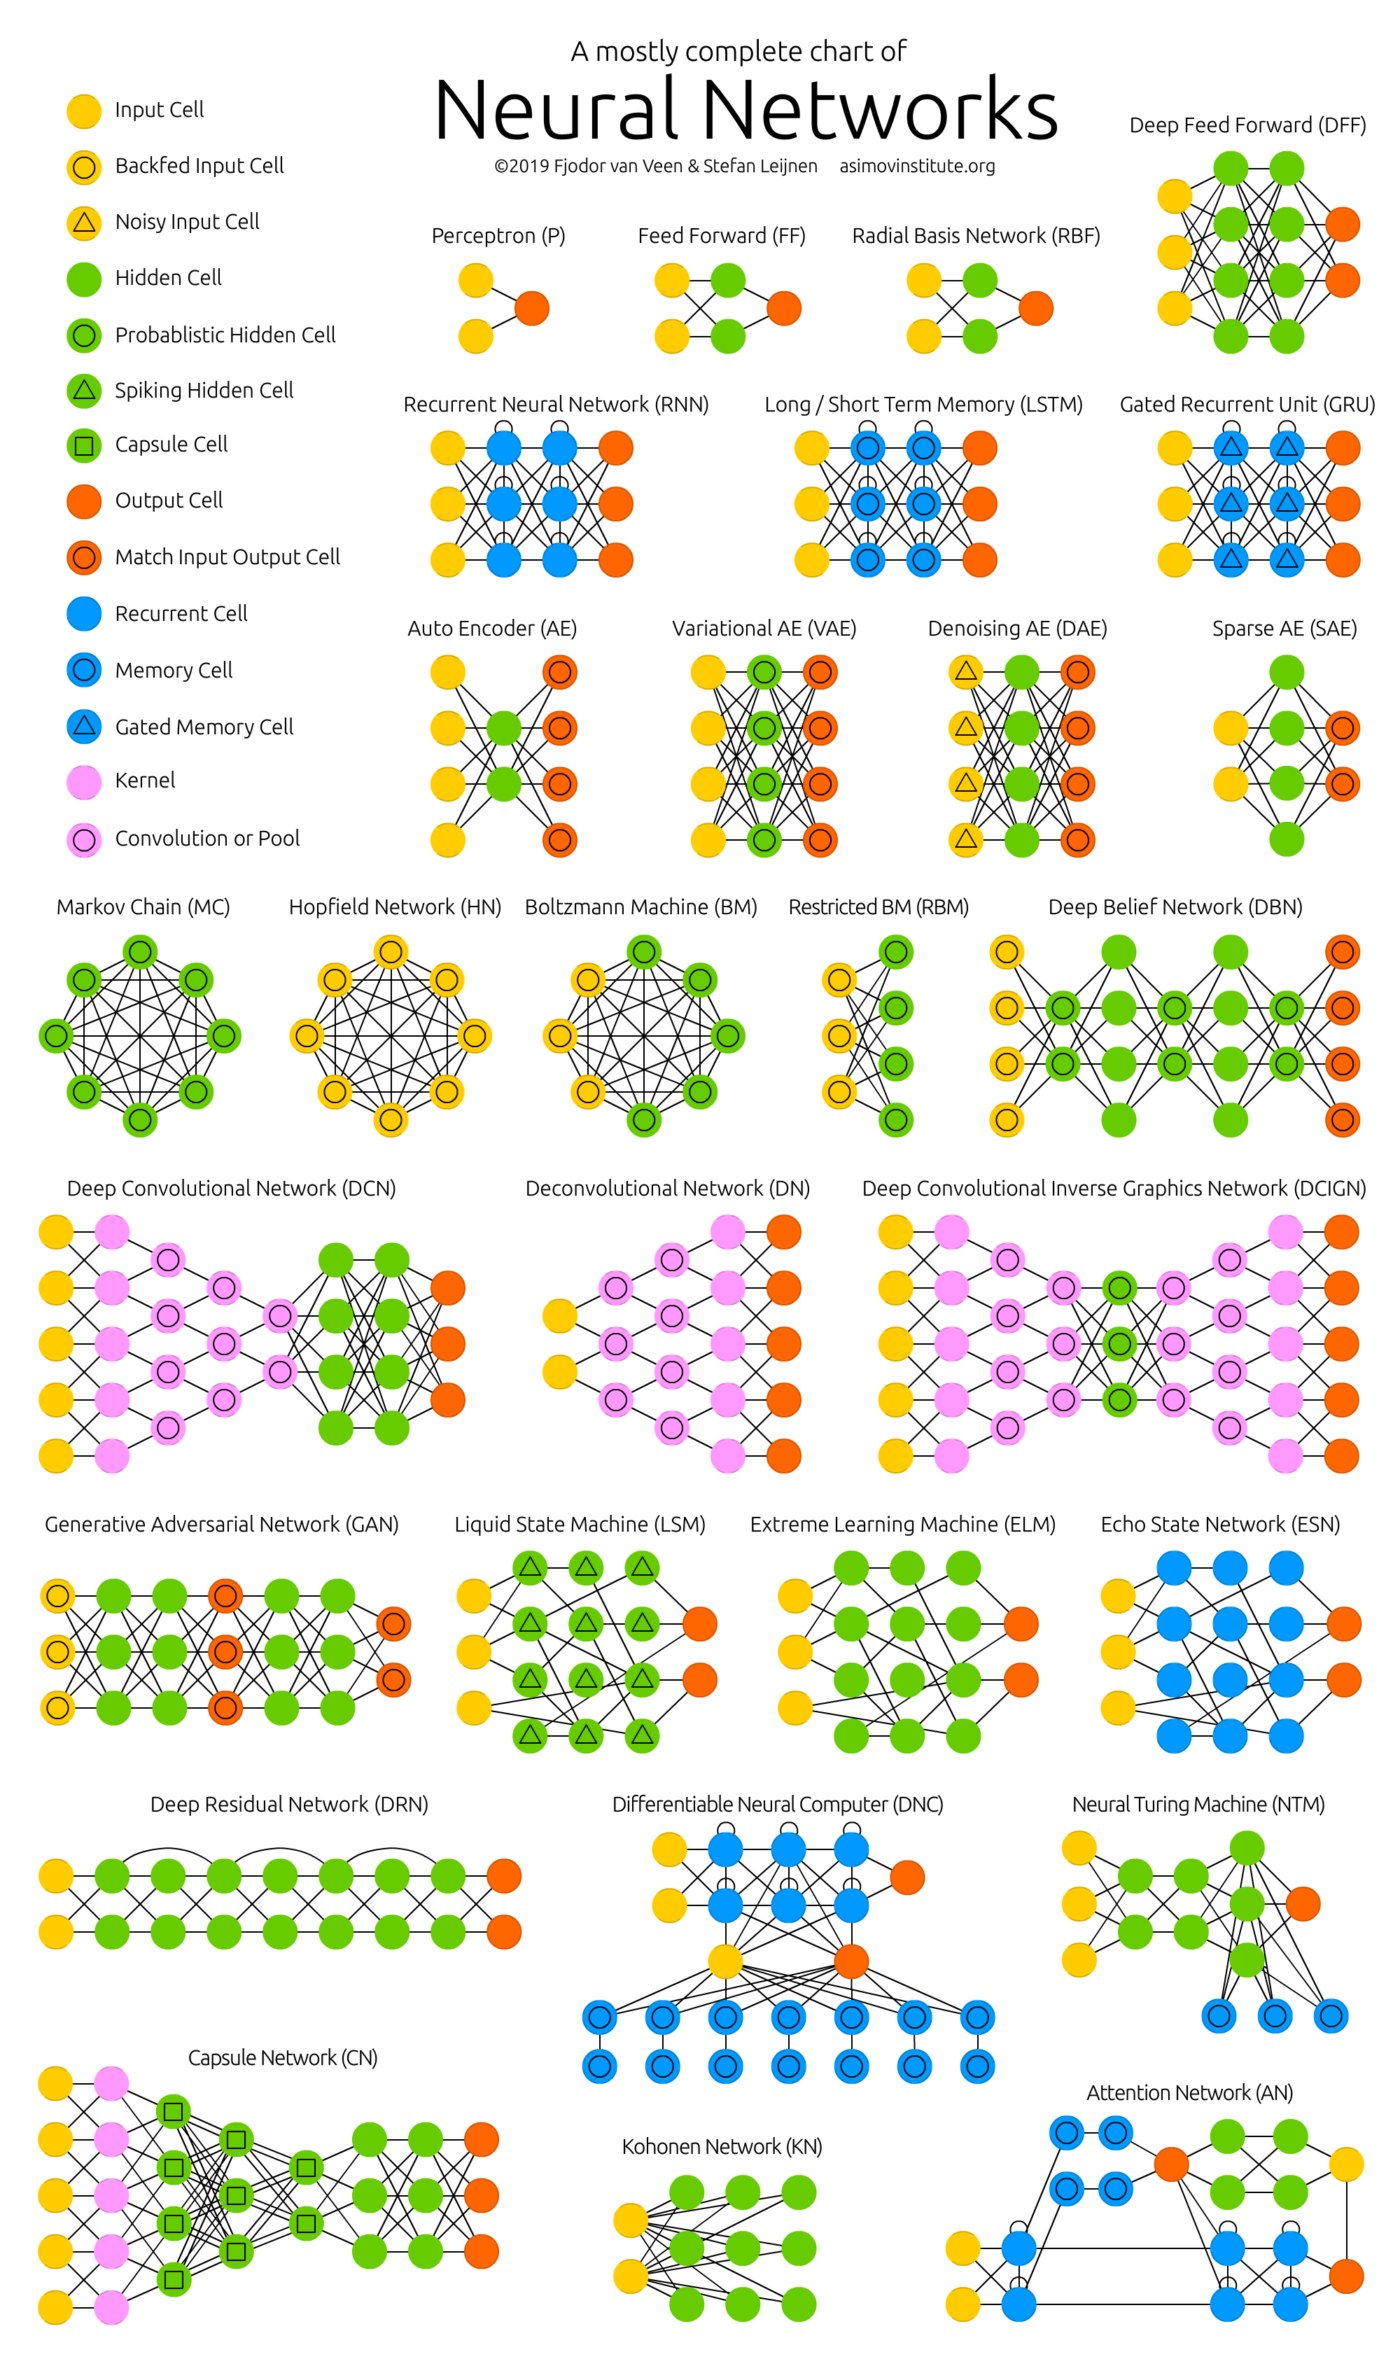
\includegraphics[width=0.7\linewidth]{imagenes/NeuralNetworkZoo20042019-1400x2380.png}
    \caption{Tipos de redes neuronales. \textit{Tomado de ASIMOV INSTITUTE about The Neural Network Zoo}
    \label{fig:my_Label})}
\end{figure}


Una red neuronal convolucional consta de diversas capas convolucionales y de pooling (submuestreo) alternadas, y al final tiene una serie de capas full-connected como una red perceptron multicapa. La entrada de una red capa convolucional suele ser, generalmente, una imagen m	x	m	x	r, donde m es tanto la altura como el ancho de la imagen y r es el número de canales. Las capas convolucionales tienen K filtros (o
kernels) cuyas dimensiones son 	n x n x q, donde n y q son elegidas por el diseñador (generalmente q suele ser igual a r). Cada filtro genera mediante convolución un mapa de rasgos o características de tamaño (m-n+1) x (m-n+1) x p, siendo p el número de filtros que se desean usar. Después cada mapa es sub-muestreado en la capa de pooling con la operación “mean pooling” o “max pooling” sobre regiones contiguas de tamaño p x p, donde p puede tomar valores desde 2 para imágenes pequeñas hasta,comúnmente, no más de 5 para imágenes grandes. Antes o después del submuestreo, se aplica una función de activación sigmoidal más un sesgo para cada mapa de rasgos \cite{duran2017redes}.

\subsection {Estructura de una Red Neuronal Convolucional}

La estructura más sencilla de una RNA se conforma de tres capas, una capa de entrada, una capa oculta y una capa de salida, donde cada neurona de una capa se conecta a todas las neuronas de la otra, conocido como \textit{Fully Connected}. En una RNC, cada capa es un bloque con tres principales variables: entrada, pesos y salida. La característica fundamental es que la salida de una capa se convierte en la entrada de la próxima, es decir, se comparten las neuronas a través de filtros que permiten extraer información de las imágenes de entrada. Este proceso es secuencial y puede ser no lineal, en cada capa se realiza una función específica \cite{lecun1998gradient}.

\begin{itemize}

\item \textbf{Capa de entrada:} La capa de entrada en una red neuronal convolucional es la imagen de la base de datos que usaremos para el entrenamiento. 

\begin{figure}[H]
    \centering
    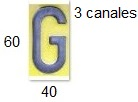
\includegraphics[width=0.4\linewidth]{imagenes/imagen_entrada.jpg}
    \caption{Imagen entrada red neuronal convolucional
    \label{fig:imagen_entrada}}
\end{figure}

\item \textbf{Capa convolucional:}Esta capa es el núcleo de las redes neuronales convolucionales. Los parámetros de esta capa consisten en un conjunto de filtros de aprendizaje, los cuales tiene un campo receptivo muy pequeño. En el paso hacia delante de aprendizaje, cada filtro se convoluciona con todo el campo de visión produciendo un mapa de características. Cada elemento del mapa de características puede interpretarse como la salida de una neurona que extrae información de una pequeña región de la entrada y comparte parámetros con neuronas que se encuentran en el mismo mapa \cite{bouvrie2006notes}. En general, el mapa de características de una capa está dado por: 

\begin{center}
    $Y_{j}^l = f(\sum_{i\in M_{j}}y_{i}^{l-1}k_{ji}^{l-1} + b_{j})$
\end{center}

Donde $M_{j}$ representa el conjunto de entradas seleccionadas y el superíndice l representa la capa actual. Cada mapeo de salida tiene un sesgo diferente. La convolución proporciona facilidad para trabajar con entradas de tamaño variable.    

La ventaja es que el mismo filtro sirve para extraer la misma característica en cualquier parte de la entrada, con esto que consigue reducir el número de conexiones y el número de parámetros a entrenar en comparación con una red multicapa de conexión total.

La fase convolucional aplicar\'a un filtro que es una pequeña matriz de píxeles dentro de la imagen. El filtro se moverá a lo largo y ancho de la imagen de entrada con dimensiones comúnmente de 3 x 3 o 5 x 5. Significa que la red desliza estas ventanas a través de toda la imagen de entrada y calcula la convolución que da como resultado una matriz que se denomina mapa de características.

\begin{figure}[H]
\centering
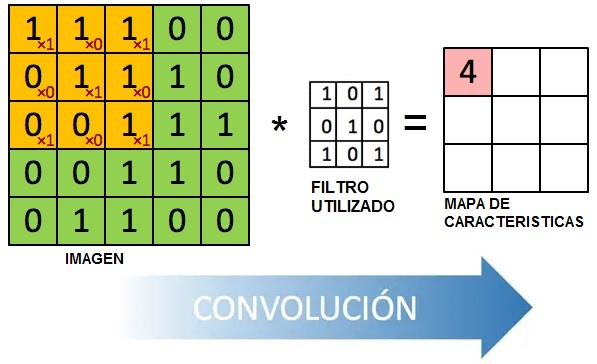
\includegraphics[width=0.5\linewidth]{imagenes/OPERACION_1.jpg}
\caption{Operación convolución}
\label{fig:OPERACION_1}
\end{figure}

En la figura \ref{fig:OPERACION_1} se ha tomado una submatriz de la imagen de entrada, con unas dimensiones igual al filtro, es decir, 3 x 3, donde las componentes son $X_{11}, X_{12}, X_{13}, X_{21}, X_{22}, X_{23}, X_{31}, X_{32}, X_{33}$ que se operan con el filtro, de la siguiente forma: $(1\times1) + (1\times0) + (1\times1) + (0\times0) + (1\times1) + (1\times0) + (0\times1) + (0\times0) + (1\times1) = 4 $ el filtro se desplaza en toda la imagen y obtenemos el mapa de características, así: 

\begin{figure}[H]
\centering
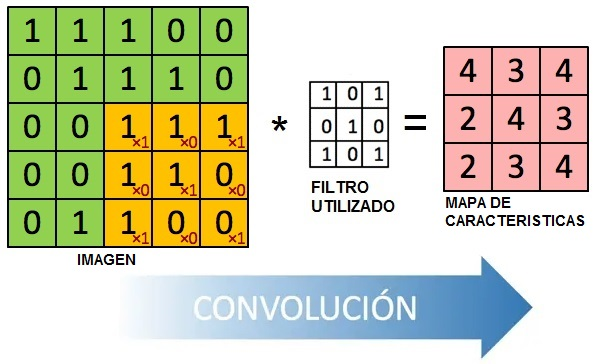
\includegraphics[width=0.4\linewidth]{imagenes/OPERACION_2.jpg}
\caption{Operación convolución}
\label{fig:OPERACION_2}
\end{figure}

\textbf{En la figura \ref{fig:OPERACION_2}} muestra como se obtiene la última componente del mapa de características, haciendo uso de $X_{33}$, $X_{34}$, $X_{35}$, $X_{43}$, $X_{44}$, $X_{45}$, $X_{53}$, $X_{54}$, $X_{55}$ de la imagen,  operado con el filtro, así: $(1\times1) + (1\times0) + (1\times1) + (1\times0) + (1\times1) + (0\times0) + (1\times1) + (0\times0) + (0\times1) = 4 $ se debe resaltar que después de esta operación el tamaño de la imagen de entrada se reduce.


En este trabajo haremos uso de imágenes de 1 y 3 canales(RGB), donde el proceso de convolución es diferente, puesto que se hace uso de los 3 filtros o kernel a la vez, en la figura \ref{fig:OPERACION1_3_CANALES} ilustramos este procedimiento.

\begin{figure}[H]
\centering
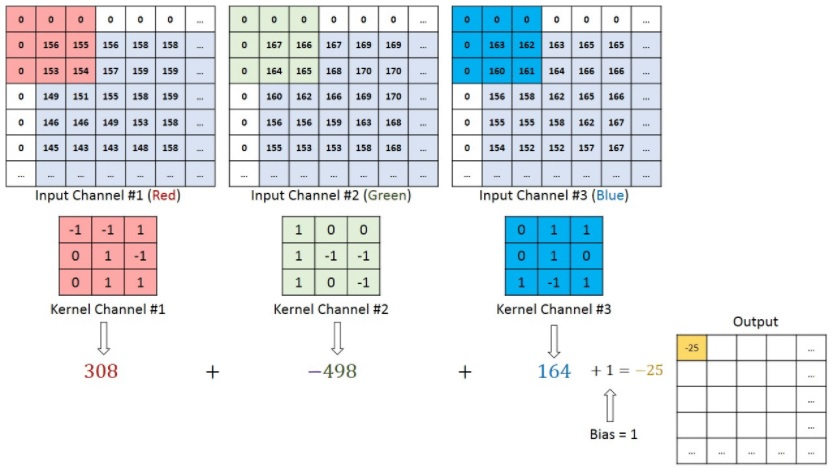
\includegraphics[width=0.8\linewidth]{imagenes/OPERACION1_3_CANALES.jpg}
\caption{Operación convolución con 3 canales RGB}
\label{fig:OPERACION1_3_CANALES}
\end{figure}
\textbf{La figura \ref{fig:OPERACION1_3_CANALES}} representa las 3 matrices para cada uno de los canales de una imagen RGB, donde se aplicada la operación de convolución con 3 filtros, donde los resultados son sumados entre si, anexando el bias.

Es importante tener en cuenta, que la imagen de salida al aplicar el filtro se reduce, comúnmente a partir del Stride con zancada 1, que tiene que ver con el desplazamiento que tiene el filtro en la matriz de entrada, si la zancada es dos, se moverá cada 2 píxeles y así sucesivamente, si queremos que la imagen de salida permanezca con los mismo píxeles de entrada, debemos hacer uso del relleno que resuelve este problema, Ren et \textit{al} \cite{Ren_2017}.

\begin{figure}[H]
\centering
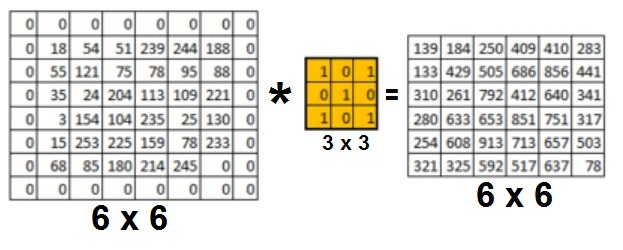
\includegraphics[width=0.5\linewidth]{imagenes/relleno.jpg}
\caption{Relleno}
\label{fig:RELLENO}
\end{figure}

\item \textbf{Capa ReLu:} El objetivo en esta capa es introducir la no linealidad, lo que significa que podemos propagar fácilmente los errores hacia atrás y tener múltiples capas de neuronas activadas por la función ReLU en nuestra red, Shaoqing et \textit{al} \cite{DBLP:journals/corr/RenHG015}. Esta función de activación se define como:\\  

R(Z) = max(0,z) = $\bigl\{\begin{array}{ccc}
    0 & para & Z<0\\
    Z & para & Z\geq 0
\end{array}$ , gráficamente es:

\begin{figure}[H]
\centering
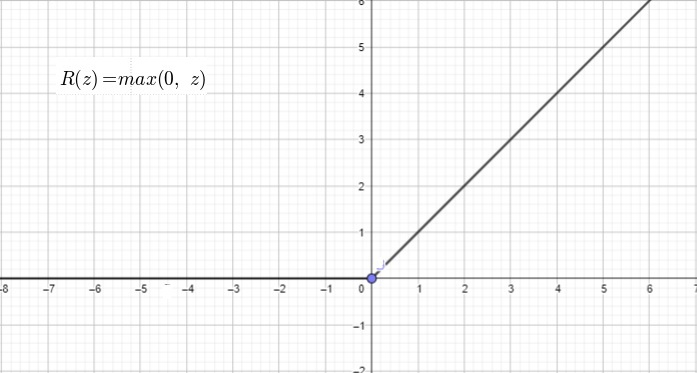
\includegraphics[width=0.7\linewidth]{imagenes/funcion_Relu.jpg}
\caption{Función de activación ReLu}
\label{fig:función_relu}
\end{figure}

Esta función se usa para permitir la no linealidad, en este componente se reemplazan los valores negativos de los píxeles por cero, tal y como se muestra en la figura \ref{fig:Relu}

\begin{figure}[H]
\centering
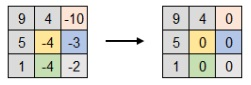
\includegraphics[width=0.7\linewidth]{imagenes/Relu.jpg}
\caption{Aplicación de la función de activación ReLu}
\label{fig:Relu}
\end{figure}

\item \textbf{Capa de submuestreo:} Se coloca después de la primera capa convolucional-ReLu con el fin de disminuir el tamaño de los datos. La operación que se realiza es mean-pooling(AVEPOOL) o comúnmente max-pooling de dimensión $s_{2}$, esta última tiene una salida:

\begin{center}
 $Y_{h}^{l} = Maxpool(Y_{h}^{l-1},s_{2} )$   
\end{center}

Esta capa reduce la cantidad de información que la capa convolucional generó para cada característica y mantiene la información más esencial (el proceso de las capas convolucionales y de agrupación generalmente se repite varias veces) \cite{pacheco2017identificacion}.

\begin{figure}[H]
\centering
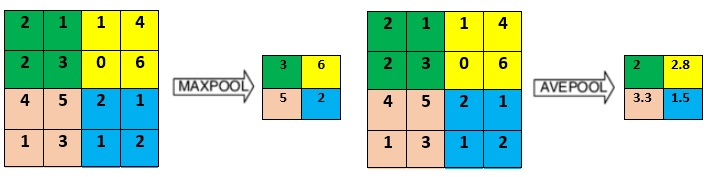
\includegraphics[width=0.7\linewidth]{imagenes/maxpooling.jpg}
\caption{Operación de max-pooling y de average-pooling}
\label{fig:Maxpooling}
\end{figure}

\textbf{La figura \ref{fig:Maxpooling}} evidencia la operación maxpooling y la operación average-pooling, la primera consiste en elegir de las componentes $X_{11}$, $X_{12}$, $X_{21}$, $X_{22}$, el máximo valor, en ese caso escogemos la componente $X_{22}$, lo mismo sucede con las componentes $X_{13}, X_{14}, X_{23}, X_{24}$ se escoge la componente $X_{24}$ ,así hacemos hasta completar las cuatro componentes del filtro 2 x 2, teniendo en cuenta que la imagen de entrada es de 4 x 4 píxeles y aplicamos un stride 2. Averagepooling consiste en hallar en este caso el promedio de las 4 componentes agrupadas anteriormente, a diferencia del máximo valor como en el caso antes mencionado. 

\item Capa de entrada totalmente conectada: “aplana” las salidas generadas por las capas anteriores para convertirlas en un solo vector que se puede usar como entrada para la siguiente capa.
\item Capa totalmente conectada: aplica pesos sobre la entrada generada por el análisis de características para predecir una etiqueta precisa.


\item \textbf{Capa Softmax o Rectified Lineal Unit:} La función Softmax transforma las salidas a una representación en forma de probabilidades para así determinar una clase para la imagen, la suma de todas las probabilidades de las salidas es igual 1.

La función esta definida como: $f(z)_j=\frac{e^{z_j}}{\sum\limits_{k=1}^{K}e^{z_k}}$, 
 donde \textit{Z} es una vector de entrada que arrojará por medio de la función de activación softmax las probabilidades para cada clase. En la figura \ref{fig:red_cov_digito_7} se resalta en un óvalo rojo la capa softmax con los valores entre 0-1 asignados a cada clase, donde la de mayor probabilidad pertenece a la clase 7.

\end{itemize}

\begin{figure}[H]
    \centering
    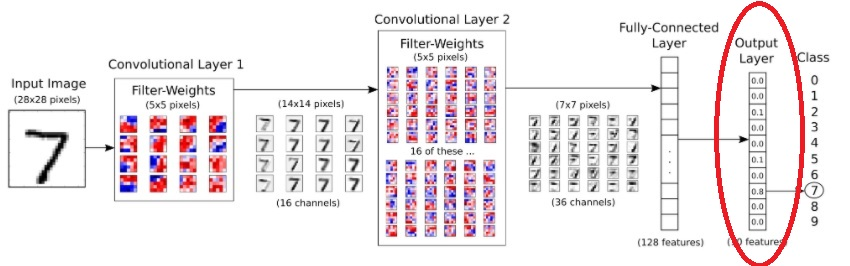
\includegraphics[width=1\linewidth]{imagenes/red_cov_digito_7.jpg}
    \caption{Arquitectura de una Red Neuronal Convolucional - RNC}
    \label{fig:red_cov_digito_7}
\end{figure}

La arquitectura de una RNC, figura \ref{fig:red_cov_digito_7} es un factor clave para determinar su rendimiento y eficiencia. La forma en que se estructuran las capas, qué elementos se usan en cada capa y cómo se diseñan a menudo afectará la velocidad y precisión con la que puede realizar diversas tareas.\\

\subsection{Evaluación del modelo de red neuronal convolucional}

\item \textbf{Matriz de confusión:} En el campo de la inteligencia artificial  y el aprendizaje automático una matriz de confusión es una herramienta que permite visualizar el desempeño de un algoritmo  de aprendizaje supervisado. Cada columna de la matriz representa el número de predicciones de cada clase, mientras que cada fila representa a las instancias en la clase real., o sea en términos prácticos nos permite ver  qué tipos de aciertos y errores está teniendo nuestro modelo a la hora de pasar por el proceso de aprendizaje con los datos, Danjuma et \textit{al} \cite{danjuma2015performance}

\begin{table}[H]
\begin{center}
\begin{tabular}{ll|c|c|}
\cline{3-4}
                   &  & \multicolumn{2}{c|}{\textbf{Categorías predichas}}\\\cline{3-4}
                                & \textbf{} & \textbf{Positivos} & \textbf{Negativos}                                                    \\ \hline 
      
\multicolumn{1}{|c|}{\multirow{2}{*}{\textbf{\begin{tabular}[c]{@{}c@{}}\\Categorías \\ verdaderas\end{tabular}}}} & \multicolumn{1}{c|}{\textbf{Positivos}} & \begin{tabular}[c]{@{}c@{}}Verdaderos\\ positivos\\ (VP)\end{tabular} & \begin{tabular}[c]{@{}c@{}}Falsos \\ negativos\\ (FN)\end{tabular}    \\ \cline{2-4} 
\multicolumn{1}{|c|}{}                                                                                           & \multicolumn{1}{c|}{\textbf{Negativos}} & \begin{tabular}[c]{@{}c@{}}Falsos\\ positivos\\ (FP)\end{tabular}     & \begin{tabular}[c]{@{}c@{}}Verdaderos\\ negativos\\ (VN)\end{tabular} \\ \hline
\label{tab:Matriz confusion Binaria}
\end{tabular}
\caption{Matriz de confusión Binaria}
\end{center}
\end{table}

Los valores correspondientes a la matriz de confusión son:

\begin{itemize}
    \item \textbf{Verdaderos Positivos(VP):}Es el número de predicciones correctas de clase positiva.
    \item \textbf{Verdaderos Negativos(VN):} Es el número de predicciones correctas de clase negativa.
    \item \textbf{Falsos Positivos(FP):}Es el número de predicciones incorrectas de clase positiva 
    \item \textbf{Falsos Negativos(FN):}Es el número de predicciones incorrectas de clase negativa 
\end{itemize}

\subsubsection*{Métricas de evaluación}\label{sec:metricas1}
\begin{itemize}
     \item \textbf{La Exactitud}: Está relacionada con el sesgo de una estimación y representa la proporción de clasificaciones predichas de manera correcta sobre el total de instancias, Borja \cite{borja2020estandarizacion}.\\ 
    \begin{center}
    $ACC = \frac{VP + VN}{VP + FP + FN + VN}$
    \end{center}
    \item \textbf{La Precisión}: Esta métrica se refiere a la dispersión del conjunto de valores obtenidos a partir de mediciones repetidas de una magnitud, cuanto menor es la dispersión mayor la precisión. Se representa por la proporción entre el número de predicciones correctas (tanto positivas como negativas) y el total de predicciones.En forma práctica es  el porcentaje de casos positivos detectados, Danjuma \cite{danjuma2015performance}.
     \begin{center}
    $PRE = \frac{VP}{VP + FP}$
    \end{center}
    \item \textbf{La Sensibilidad}Es la proporción de casos positivos que fueron correctamente identificadas por el algoritmo.
    \begin{center}
    $REC = \frac{VP}{VP + FN}$
    \end{center}
    
    \item \textbf{La Especificidad} Se trata de los casos negativos que el algoritmo ha clasificado correctamente.  Expresa cuan bien puede el modelo detectar esa clase.
     \begin{center}
    $ESP = \frac{VN}{VN + FP}$
    \end{center}
    
    \item \textbf{Valor-F} Esta métrica además de ser muy empleada, es muy importante, ya que nos resume la precisión y sensibilidad en una sola métrica y es de gran utilidad cuando la distribución de las clases es desigual.
    \begin{center}
    $Valor-F = 2\times \frac{Sensibilidad \times Precision}{Sensibilidad + Precision}$
    \end{center}
    
    Conforme a estas nuevas métricas podemos obtener cuatro casos posibles para cada clase:
    \begin{itemize}
    \begin{itemize}
        \item[$\rightarrow$] Alta precisión y alto recall nos indica que el modelo maneja perfectamente esa clase.
        \item[$\rightarrow$] Alta precisión y bajo recall nos indica que el modelo no detecta la clase muy bien, pero cuando lo hace es altamente confiable.
        \item[$\rightarrow$] Baja precisión y alto recall nos indica que el modelo detecta bien la clase,  pero también incluye muestras de la otra clase.
       \item[$\rightarrow$] Baja precisión y bajo recall nos indica que el modelo no logra clasificar la clase correctamente.
    \end{itemize}
    \end{itemize}
    
Es importante tener en cuenta que cuando tenemos un “dataset” con desequilibrio, suele ocurrir que obtenemos un alto valor de precisión en la clase Mayoritaria y un bajo recall en la clase Minoritaria, Danjuma et \textit{al} \cite{danjuma2015performance}.
\end{itemize} \\

La tabla \ref{tab:Matriz de confusion con otras metricas de evaluacion} nos resume la matriz de confusión de una categoría dicotómica y las métricas de evaluación:

\begin{table}[H]
    \centering
    \resizebox{\textwidth}{!}{
    \begin{tabular}{|c|c|c|c|c|c|}
    \hline
\multicolumn{2}{|l|}{\multirow{2}{*}{\textbf{\begin{tabular}[c]{@{}c@{}}Matriz de confusión\end{tabular}}}} & \multicolumn{2}{c|}{\multirow{1}{*}{\textbf{\begin{tabular}[c]{@{}c@{}}Predichos\end{tabular}}}} & \multicolumn{2}{l|}{} \\ \cline{3-4} \multicolumn{1}{|}{}   &   & Positivo & Negativo & \multicolumn{1}{|}{} &  \\ \hline
\multirow{2}{*}{Categorías Verdaderas} & Positivo & \textbf{VP} & \textbf{FP} & Precisión & \textbf{VP/(VP+FP)} \\ \cline{2-6}
         & Negativo  & \textbf{FN} & \textbf{VN} & Verdadero negativo & \textbf{VN/(VN+FN)} \\ \hline
\multicolumn{2}{|l|}{} & Sensibilidad & Especificidad & \multicolumn{2}{c|}{\multirow{2}{*}{\textbf{\begin{tabular}[c]{@{}c@{}}Exactitud=(VP+VN)/(VP+FP+FN+VN)\end{tabular}}}} \\ \cline{3-4}
\multicolumn{2}{|l|}{} & \textbf{VP/(VP+FN)} & \textbf{VN/(VN+FP)} &  \multicolumn{2}{l|}{} \\ \hline
    \end{tabular}
    }
    \caption{Matriz de confusión con otras métricas de evaluación}
    \label{tab:Matriz de confusion con otras metricas de evaluacion}
\end{table}


\subsection{Detección de objetos}\label{sec:deteccionobjetos}
La detección de objetos es una parte integral de la visión por computadora,nos ayuda en la estimación de pose, detección de vehículos, vigilancia, entre otras cosas, la diferencia entre los  los algoritmos de clasificación y los algoritmos de detección, es que los primeros generalmente clasifican una imagen de acuerdo al las clases con las que se entrenó la red, mientras que los algoritmos de detección de objetos intentan dibujar un cuadro delimitador alrededor del objeto de interés para ubicarlo dentro de la imagen. Además, es posible que no dibuje necesariamente un solo cuadro delimitador en un caso de detección de objetos, podría haber muchos cuadros delimitadores que representen diferentes objetos de interés dentro de la imagen y no sabría cuántos de antemano, ya que depende de cada imagen, Ren et \textit{al} \cite{DBLP:journals/corr/RenHG015}.


Existe varios tipos de R-CNN, cada una con características diferentes, pero tratando de optimizar, acelerar o mejorar los resultados de detección de objetos, Taguri et \textit{al} \cite{Taguri_missinglink.ai}.\\ 
La tabla \ref{tab:Tipos de R-cnn} especifica alguna de estas redes neuronales convolucionales: 

\begin{table}[H]
\begin{center}
\resizebox{0.65\textwidth}{!}{
\begin{tabular}{ | l | p{5cm} | p{5cm} |}
\hline
    TIPO DE R-CNN & CARACTERÍSTICAS & LIMITACIONES \\ \hline
    R-CNN & Esta red hace una búsqueda selectiva para identificar la región de interés, exactamente 2000 por medio del algoritmo de búsqueda selectiva, que propone muchas regiones candidatas que de acuerdo a su similitud se van unificando hasta lograr esta cantidad, que sera procesada por la red neuronal convolucional para realizar la extracción de características de cada región de forma independiente para su clasificación. & La capacitación se considera muy costosa y lenta por la cantidad de procesos internos, especialmente la identificación de una cantidad significativa de regiones de interés, además se requiere de 3 modelos internos por separado sin mucho calculo en común, y el uso no se puede hacer en tiempo real, debido al tiempo que tarda en procesar cada imagen, alrededor de 47 segundos.\\ \hline
    Fast R-CNN & Cada imagen se trasmite una sola vez a la CNN y esta genera una mapa de características, que permite identificar las regiones propuestas y se deforman en cuadrados  delimitadores. Se resalta que esta técnica es mucho más rápida que R-CNN en tiempo de entrenamiento y prueba  & La búsqueda selectiva de las regiones es lenta y, por lo tanto, el tiempo de cálculo es muy elevado, adem\'as las propuestas de región se generan por separado utilizando un modelo diferente.\\ \hline
    Faster R-CNN & Esta red usa un modelo unificado compuesto por RPN (red de propuesta de región) y R-CNN rápido con capas de características convolucionales compartidas, que facilta el proceso, ya que elimina el algoritmo de búsqueda selectiva y permite que la red aprenda las propuestas de la región, En lugar de usar un algoritmo de búsqueda selectiva en el mapa de características para identificar las propuestas de región como hace Fast CNN, se usa una red separada para predecir las propuestas de región. & Las propuestas de objetos con RPN requieren mucho tiempo, lo que implica que el rendimiento de todo el sistema se ve afectado por tal motivo  \\
    \hline
    \end{tabular}
    }
    \label{tab:Tipos de R-cnn}
\end{center}
\end{table}

\item \textbf{Arquitectura de Faster R-CNN:}\label{sec:Faster}

\begin{figure}[H]
    \centering
    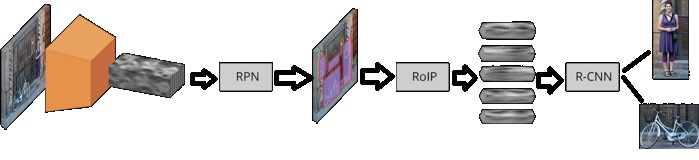
\includegraphics[width=0.8\linewidth]{imagenes/Arquitectura_faster.jpg}
    \caption{Arquitectura de una Faster R-CNN}
    \label{fig:Arquitectura_Faster}
\end{figure}

la figura \ref{fig:Arquitectura_Faster} muestra que la entrada de esta red es una imagen donde se extraen las características por medio de una red neuronal convolucional, para luego usar una Region Proposal Network (RPN), que permite generar varias propuestas de regiones, que se conocen como Bounding Box, estos cuadros delimitadores se reforman utilizando una capa de agrupación de regiones de interés (RoIP), que posteriormente me permite clasificar la imagen dentro de la región propuesta y predecir los valores de desplazamiento con una R-CNN para los cuadros delimitadores, Ren et \textit{al} \cite{Ren_2017}.

Shaoqing et \textit{al} \cite{DBLP:journals/corr/RenHG015} indica que después de extraer las características por medio de una CNN, los pasos que siguen en la Faster R-CNN son:

\begin{itemize}
    \item \textbf{Funcionamiento Region Proposal Network (RPN):} Finalizado el proceso de extracción de características en la última capa de convolución de la CNN, la \textbf{RPN} ejecuta una ventana deslizante sobre el mapa de características, generalmente con dimensiones n x n, generando $n^2$ anclajes/cajas con igual centro ($X_1, Y_1$) pero con \textbf{n} aspectos y \textbf{n} escalas diferentes. 
    
    \begin{figure}[H]
    \centering
    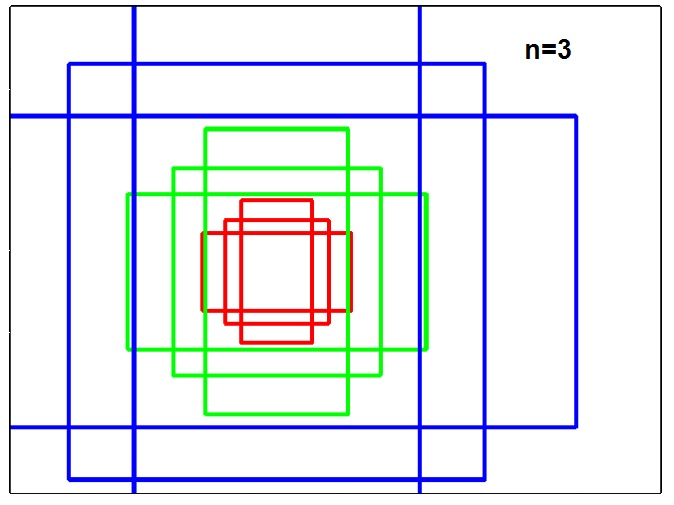
\includegraphics[width=.6\linewidth]{imagenes/anclajes.jpg}
    \caption{Propuestas de anclajes}
    \label{fig:Anclajes}
\end{figure}
    
    Para cada uno de estos anclajes, se calcula un valor p ∗ que indica cuánto se superponen estos anclajes con los cuadros delimitadores(GTBox), así:
    
    IoU = $\frac{A\cap GT}{A \cup GT}$ = $\bigl\{\begin{array}{ccc}
    > 0.7 = Hay & objeto & \\
    < 0.3 = No & hay & objeto
\end{array}$ 
    
IoU = $ \frac{Anclaje \cap GTBox}{Anclaje \cup GTBox}  $
    
    \item \textbf{Funcionamiento de la capa de agrupación de ROI Pooling:} Esta capa recibe muchas propuestas de regiones con tamaños diferentes, extraer características para cada una de esas propuestas  y reduce los mapas de características al mismo tamaño.
    \item \textbf{Funcionamiento Capa final R-CNN:} Después de obtener los mapas de características de \textbf{ROI-P}, estas se usan para la clasificación, a partir de la red neuronal convolucional basada en regiones (R-CNN),intenta imitar las etapas finales de las CNN de clasificación en las que se utiliza una capa completamente conectada para generar una puntuación para cada clase de objeto posible.
\end{itemize}


\subsection{Librerías para Modelos pre-entrenados} 
Existen múltiples librerías de código abierto usadas para \textit{Deep Learning} en lenguaje Python. A continuación, detallamos las usadas en el presente trabajo: 

\Item \textbf{TensorFlow}: Es una interfaz para expresar algoritmos de aprendizaje automático y una implementación para ejecutar dichos algoritmos. Un cálculo expresado con TensorFlow se puede ejecutar con poco o ningún cambio en una amplia variedad de sistemas computacionales heterogéneos, \cite{tensorflow2015-whitepaper}. Su sistema es flexible y se puede utilizar para expresar una amplia variedad de algoritmos, incluidos los algoritmos de entrenamiento e inferencia para modelos de redes neuronales profundas, y se ha utilizado para realizar investigaciones y desplegar sistemas de aprendizaje automático en producción en más de una docena de áreas de ciencias de la computación y otros campos, incluidos el reconocimiento de voz, la visión por computadora, la robótica, la recuperación de información, el procesamiento del lenguaje natural, la extracción de información geográfica y el descubrimiento computacional de drogas. TensorFlow se lanzó como un paquete de código abierto bajo la licencia Apache 2.0 en noviembre de 2015 y están disponibles en www.tensorflow.org. El uso de TensorFlow como una maquina de calculo en paralelo aplicado a problemas de clasificación de imágenes con metodologías de Redes neuronales, es una de las aplicaciones mas recientes de la Inteligencia Artificial.\\

\Item \textbf{OpenCV}\label{opencv}: Es una librería de visión artificial desarrollada por Intel y actualmente publicada bajo licencia BSD, que cuenta con más de medio millar de algoritmos optimizados para realizar las principales tareas de visión artificial, como el procesamiento de imágenes, detección de características o reconocimiento de objetos. La librería cuenta además con diferentes algoritmos de aprendizaje de máquina como máquinas de soporte de vectores (SVM), Naïve Bayes o KNN entre otros, \cite{opencv_library}
Está escrita en C++, es multiplataforma y cuenta con interfaces para trabajar con lenguajes como Java o Python. La gran cantidad de algoritmos disponibles, su velocidad de ejecución y la extensa comunidad de usuarios de que dispone, hacen de OpenCV una herramienta indispensable para desarrollar sistemas de visión artificial basados en software de código abierto.

\subsection{Aplicativos comerciales de reconocimiento de matrículas}

\begin{itemize}
    \item NEC: El analizador de matriculas de vehículos de NEC es uno de los sistemas ANPR, lideres en el mundo. Utiliza algoritmos de alta velocidad y precisión de tipo GLVQ ("\textit{Generalized Learning Vector Quantization}" que en español significa  Cuantización del vector de aprendizaje generalizado).El reconocimiento de matriculas de NEC es altamente preciso incluso en condiciones climáticas adversas. Extrae matriculas vehiculares inclinadas/desplazadas/rotadas Trabaja con imágenes borrosas, con ruido o poco contraste\cite{SoftwareNEC}.
    \item VPAR – Librería de reconocimiento de placas. Neural Labs presenta el software definitivo en el campo del reconocimiento automático de placas de vehículos. Basado en tecnología neuronal propia en constante evolución, proporciona al profesional de la seguridad, un sistema de detección de placas seguro, de fácil instalación e integración en cualquier sistema operativo, y lo que es más importante, con garantía de máxima fiabilidad de lectura\cite{SoftwareVPAR}.
    \item OpenALPR es una biblioteca de reconocimiento automático de matrículas escrita en el lenguaje de programación C++. El software se distribuye en dos versiones: una de código abierto y otra comercial\cite{SoftwareOpen}.
    \item PlateSmart Technologies es una compañía de reconocimiento de matrículas (LPR) basada en software con sede en Oldsmar, Florida. El software independiente de la cámara de la compañía utiliza una cámara de video y una computadora para identificar y grabar placas a través de algoritmos de análisis de video. El producto principal de PlateSmart, ARES, se integra con el hardware existente para crear un sistema LPR\cite{softwarePlateSmart}.
\end{itemize}

\subsection{Bases de datos públicas para el entrenamiento de RNC y Faster R-CNN}

\subsubsection{Ckars74k}\label{Chars74k}

El conjunto de datos \textbf{Chars74k} creado por T. de Campos y M. Varma de Microsoft Research India\cite{de2012chars74k}. Este dataset cuenta con más de 74.000 imágenes de números y letras en formato PNG organizadas en tres colecciones: caracteres manuscritos, caracteres extraídos de fotografías de escenas cotidianas y caracteres generados por ordenador.

Esta última colección cuenta con más de 60.000 imágenes en escala de grises de dígitos y letras representados con diferentes fuentes y estilos (normal, negrita y cursiva), a priori idóneas para que la red CNN “aprenda” a reconocer los patrones de los distintos números y letras de las matrículas\cite{de2009chars74k}. Específicamente incluye:

\begin{itemize}
    \item 64 clases (0-9, AZ, az)
    \item 7705 caracteres obtenidos de imágenes naturales
    \item 3410 personajes dibujados a mano con una tableta
    \item 62992 caracteres sintetizados de fuentes de computadora
\end{itemize}

\subsubsection{Microsoft COCO: \textit{Common Objects in Context}}
\label{sec:coco}
También hay disponibles bases de datos de imágenes para entrenamiento y evaluación de las redes neurales profundas. Los resultados obtenidos en estas evaluaciones se comparan con los de los trabajos originales con la métrica promedio de precisión promedio (mAP). Esta métrica se calcula tomando el promedio sobre mAP calculado en cada umbral de IoU de 0.5 a 0.95, con un paso de 0.05. Las detecciones están limitadas a 100 por imagen. También se hacen algunas consideraciones sobre el tiempo de inferencia de los métodos. Algunas bases de datos son: PASCAL VOC 2007, 2012, MS COCO datasets, Google’s Open Images Dataset V4.

\textit{Common Objects in Context} - COCO, proporciona conjuntos de datos de detección, segmentación y subtitulación de objetos a gran escala \cite{lin2014microsoft}. COCO tiene varias características:

\begin{itemize}
    \item Segmentación de objetos
    \item Reconocimiento en contexto
    \item Segmentación de superpíxeles
    \item 330K imágenes ( > 200K etiquetadas)
    \item 1,5 millones de instancias de objetos
\item 80 categorías de objetos
\item 91 categorías de cosas
\item 5 subtítulos por imagen
\item 250,000 personas con puntos clave
\end{itemize}

El conjunto de datos proporciona múltiples imágenes con las anotaciones correspondientes. Una anotación contiene información sobre el cuadro delimitador y la clasificación de cada objeto en esa imagen que pertenece a una de las clases de interés de ese conjunto de datos. El conjunto de datos puede contener información para otras tareas, como la segmentación\cite{lin2014microsoft}.

\subsection{Segmentación con \textit{Python}}
 El procesamiento de imágenes que ejecuta el módulo \textit{Python} está basado en OpenCV y emplea las siguientes técnicas: 
\begin{itemize}
    \item Conversión a escala de grises: La información de color no es necesaria para el problema planteado y su eliminación facilita la detección de los caracteres de la matrícula. La función  de OpenCV que se utiliza es \textbf{cvtColor}.
    
    \item Thresholding: El thresholding o “técnica del valor umbral” es un método de binarización que permite obtener una imagen en la que quedan claramente definidos los contornos de los caracteres, facilitando el proceso de segmentación o aislamiento de las áreas que los contienen. La función  de OpenCV que se utiliza es \textbf{thresholding}.
    
    \item Desenfoque Gaussiano: Aplicar efecto de suavizado en la imagen para eliminar el ruido. En concreto, se aplica un filtro de desenfoque Gaussiano que consiste en mezclar ligeramente los niveles de gris entre píxeles adyacentes, lo que da como resultado una imagen con los bordes más suaves en la que se pierden pequeños detalles, de manera similar a lo que ocurre en las fotografías desenfocadas. La función  de OpenCV que se utiliza es \textbf{GaussianBlur}.
    
    \item Detección de contornos: Los contornos o bordes son curvas que unen conjuntos de píxeles contiguos que tienen el mismo color o intensidad. Estas curvas permiten localizar las fronteras de los objetos de la imagen, y su detección es fundamental para que un sistema de visión artificial pueda reconocer o detectar formas en una imagen. Las funciones  de OpenCV que se utilizan son \textbf{findContours} y \textbf{boundingRect}.
\end{itemize}.
